\documentclass[10pt,a4paper]{scrartcl}
\pagestyle{empty}
\usepackage{a4} % alternativ \usepackage{a4wide}
\usepackage[ngerman]{babel} % Neudeutsche Silbentrennung (mehrsprachiges Dokument)
\usepackage{parskip} % Skip indentation of first row
\usepackage{graphicx} % Graphics support
\usepackage{longtable} % Tables across several pages
\usepackage{booktabs}
\usepackage{hyperref} % Hyperlinks
\usepackage{float} % Force float position
\usepackage[automark]{scrpage2} %kopf/fusszeile
\usepackage{listings}
\usepackage[utf8x]{inputenc} % Unicode-Encoding

\linespread{1.3}

\author{Danilo Bargen, Christian Fässler, Jonas Furrer} 
\title{Systemtests\\Projekt BierIdee}

\pagestyle{scrheadings}
\ihead{SE2 Projekte} %linke Kopfzeile
\ohead{BierIdee} %rechte Kopfzeile

\begin{document}

\begin{titlepage}
	\maketitle
	\vspace{120mm}
	\thispagestyle{empty} % Don't start page numbers on this page
\end{titlepage}

\tableofcontents
\newpage

\section*{Änderungshistorie}
\begin{tabular}{p{0.1\textwidth}p{0.15\textwidth}p{0.55\textwidth}p{0.1\textwidth}}
\toprule
\textbf{Version} & \textbf{Datum} & \textbf{Änderung} & \textbf{Person} \\  
\midrule
v1.0 & 07.05.2012 & Dokument erstellt, Load Tests dokumentiert & dbargen \\  
%\hline 
%v1.1 & 28.04.2012 & Grafiken für Modellierungsvarianten eingefügt & cfaessle \\
\hline 
\bottomrule
\end{tabular} 
\newpage

\section{Vorwort}

Der Systemtest ist die Teststufe, bei der das gesamte System gegen die gesamten Anforderungen
(funktionale und nicht funktionale Anforderungen) getestet wird. Gewöhnlich findet der Test auf
einer Testumgebung statt und wird mit Testdaten durchgeführt.


\section{Funktionale Systemtests}

\subsection{Android App}

Funktionale Systemtests für Android werden mithilfe von
Robotium\footnote{\url{http://code.google.com/p/robotium/}} automatisiert umgesetzt. Sie
funktionieren grundsätzlich gleich wie die Integration Tests, werden jedoch nicht auf kleinen
Einheiten getestet. Stattdessen werden ganze Use Cases automatisiert ausgeführt und verifiziert.

Der Reallife-Einsatz der App wird durch von Entwicklern begleitete User Tests abgedeckt.

\subsection{REST API}

Da die REST API stateless ist und keine konkreten Workflows existieren, werden hier keine
funktionalen Systemtests durchgeführt, da das Testen der Funktionalität bereits durch die
Integration Tests komplett abgedeckt wird.


\section{API Load Tests}

Die Load Tests dienen dazu, die Grenzen des Testsystems auszuloten und zu sehen, ob die
gesetzten Performanceziele erreicht werden können.

Um die Load Tests durchzuführen, wurde der Service von \url{http://blitz.io/} verwendet. Die Seite
ermöglicht es, eine API mit Sprints (einfache Analyse der Seite) und Rushes (steigende Belastung
durch concurrent Requests) auszulasten. Die Auslastungstests wurden jeweils auf der
Beerlist-Ressource durchgeführt.


\subsection{50 Concurrent Users}

Um unser Ziel von 50 concurrent Users zu verifizieren, haben wir einen Rush durchgeführt, der während
60 Sekunden die Anzahl paralleler Requests von 1 auf 50 steigert und Timeouts sowie Fehler loggt.

\subsubsection*{Query}

\texttt{-p 1-50:60 http://brauhaus.nusszipfel.com:8080/beers}

\subsubsection*{Analyse}

Der Rush generierte 1'277 erfolgreiche Hits während einer Minute. Dabei wurden 7.21 MB Daten übertragen.
Die Durchschnitts-Hitrate von 20 Hits / Sekunde bedeutet eine erfolgreiche Bewältigung von ca. 1'757'055
Hits / Tag.

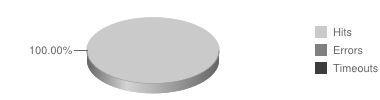
\includegraphics[scale=1]{loadtests/chart-50.png}

\subsubsection*{Response-Zeiten}

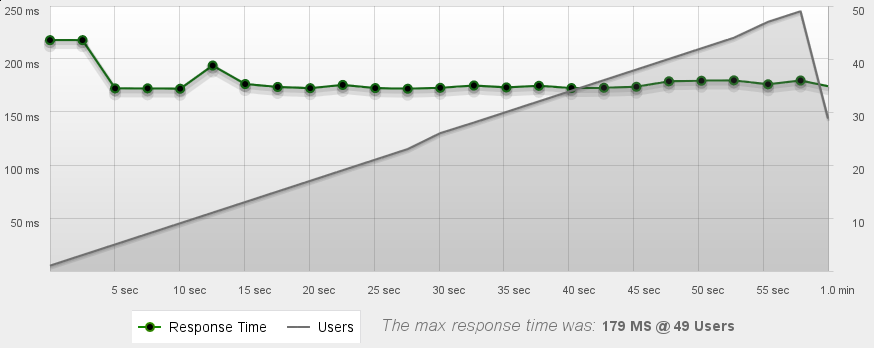
\includegraphics[width=\textwidth]{loadtests/responsetimes-50.png}

\subsubsection*{Hit Rate}

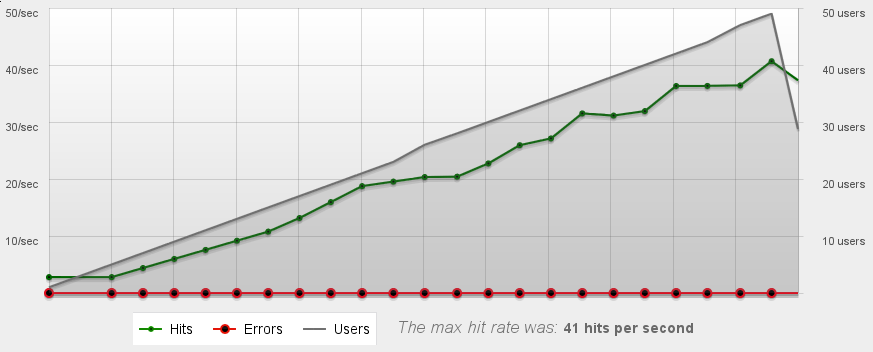
\includegraphics[width=\textwidth]{loadtests/hitrate-50.png}


\subsection{200 Concurrent Users}

Um die Grenzen des Systems zu erkennen, haben wir noch einen Test mit 200 concurrent Users
durchgeführt. Dabei wurde während 60 Sekunden die Anzahl paralleler Requests von 1 auf 200
gesteigert und die Timeouts sowie Fehler geloggt.

\subsubsection*{Query}

\texttt{-p 1-200:60 http://brauhaus.nusszipfel.com:8080/beers}

\subsubsection*{Analyse}

Der Rush generierte 2'600 erfolgreiche Hits während einer Minute. Dabei wurden 14.67 MB Daten übertragen.
Die Durchschnitts-Hitrate von 41 Hits / Sekunde entspricht ca. 1'757'055 Hits / Tag.

Es gab jedoch Probleme -- 52.42\% der User Requests resultierten in Timeouts oder Fehlern.

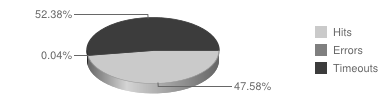
\includegraphics[scale=1]{loadtests/chart-200.png} 

\paragraph*{Fehler}

Der erste Fehler trat nach 57.72 Sekunden bei 193 concurrent Users auf. Die Fehler sind vermutlich
auf Ressourcenüberlastung zurückzuführen, wie zB ungenügend freie File Descriptors oder zu kleine
Connection Pools.

\paragraph*{Timeouts}

Der erste Timeout trat nach 22.56 Sekunden bei 76 concurrent Users auf. Die Timeout-Zeit war auf 1
Sekunde gesetzt. Man könnte die Timeouts mithilfe von Caching drastisch reduzieren.

\subsubsection*{Response-Zeiten}

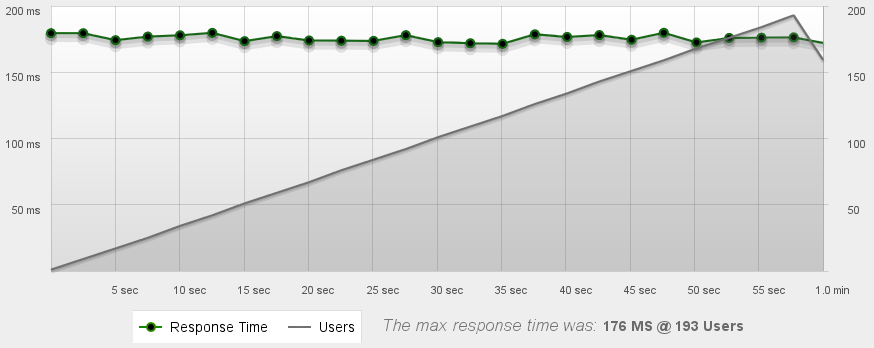
\includegraphics[width=\textwidth]{loadtests/responsetimes-200.png} 

\subsubsection*{Hit Rate}

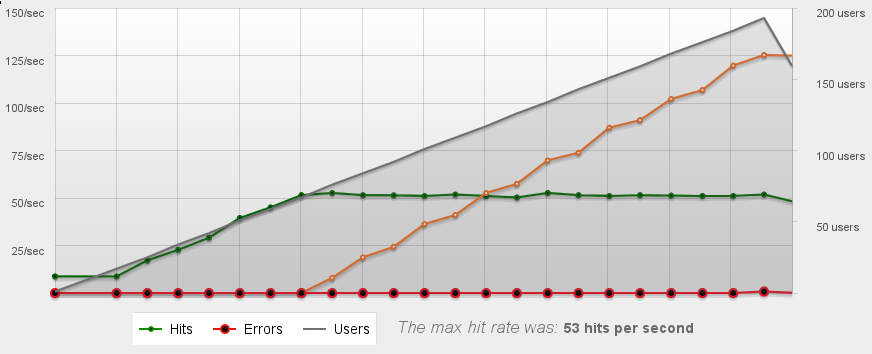
\includegraphics[width=\textwidth]{loadtests/hitrate-200.png}


\subsection{Auswertung}

Wie man am Test mit 50 gleichzeitien Benutzern sieht, können wir unser selbst gesteckte Auslastungs-Ziel
problemlos erreichen. Die maximale Response-Zeit von 179ms bei 41 Hits / Sekunde ist äusserst tief,
vor allem wenn man bedenkt dass die Requests von Virginia, USA aus erzeugt wurden. Bei dieser Menge
an Anfragen trat kein einziger Timeout oder Fehler auf.

Anders sieht es aus, wenn man die Anzahl paralleler Benutzer erhöht. Wie man in den Diagrammen sehr
gut sehen kann, kann der Server ziemlich genau 50 Hits pro Sekunde bewältigen. Danach bleibt die
Anzahl erfolgreich beantworteter Requests konstant, obwohl die Gesamtanzahl Hits weiterhin erhöht
wurde. Die Anzahl der Timeouts steigt parallel zur Erhöhung der parallelen User. Dies heisst, dass
die Grenze unseres Systems bei ziemlich genau \textbf{76 gleichzeitigen Benutzern} liegt. Dies ist
ein sehr guter Wert, wenn man bedenkt dass auf dem Server bisher keinerlei Caching o.ä. eingerichtet
wurde.

Auch bei 200 gleichzeitigen Benutzern gab es lediglich viele Timeouts, jedoch keine kritischen
Fehler. Das bedeutet, dass die Benutzung der App bei einer solchen Menge an Benutzern zwar sehr
langsam wäre, jedoch in keinen Fehlermeldungen resultieren würde.


\end{document}
